\documentclass{article}
\usepackage{tikz}
\usepackage[a4paper]{geometry}
\usepackage{fancyhdr}
\pagestyle{fancy}
\lhead{Wahrscheinlichkeiten Darstellen}
\rhead{August 2025}
\begin{document}
 

\section{Wahrscheinlichkeiten Darstellen} 
\subsection{Baumdiagramme}
\begin{minipage}{\dimexpr\linewidth-5cm} 
Ein Baumdiagramm ist ein Diagramm, welches von einem Ausgangspunkt aus die direkten Folgen verbindet, diese können wiederum ein eigener Ausgangspunkt, oder ein Endergebnis sein. Auf den Verbindungslinien, steht die Wahrscheinlichkeit, dass basierend auf dem Ausgangspunkt ein bestimmtes Ereigniss eintritt. Die Wahrscheinlichkeit, dass ein Endergebnis eintritt, ist das Produkt aller Wahrscheinlichkeiten der Pfade, welche dazu geführt hatten, dass dieses eintritt.
\end{minipage}
\hfill
\begin{minipage}{5cm}
 \center
 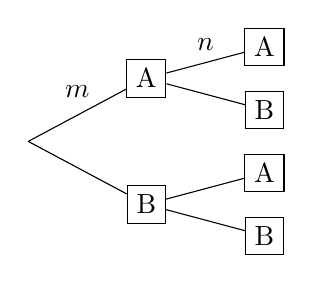
\begin{tikzpicture}
    \node[draw] (a) at (1.5,0.8) {A};
    \node[draw] (b) at (1.5,-0.8) {B};
 
    \node[draw] (aa) at (3,1.2) {A};
    \node[draw] (ab) at (3,0.4) {B};
 
    \node[draw] (ba) at (3,-0.4) {A};
    \node[draw] (bb) at (3,-1.2) {B};
    \draw (0, 0) -- (a) node[midway, above, yshift=3pt] {$m$}; 
    \draw (0, 0) -- (b);
 
    \draw (a) -- (aa) node[midway, above, yshift=1pt] {$n$};  
    \draw (a) -- (ab);  
    \draw (b) -- (ba);  
    \draw (b) -- (bb); 
 \end{tikzpicture} 
\end{minipage}
\vspace{-0.35em} \newline
Das Beispielbaumdiagramm, rechts, zeigt, dass vom Ausgangspunkt aus die Chance, dass A eintritt, bei $m$ liegt. Ist A bereits einmal eingetreten, ist liegt die Wahrscheinlichkeit dass es erneut eintritt bei $n$. Somit ist $P(A, A) = m \cdot n$ 
 
\subsection{Vierfeldertafel}
\begin{minipage}{\dimexpr\linewidth-8cm} 
 Eine Vierfeldertafel ist eine art Tabelle, welche jeweils in ihren Zeilen und Spalten die wahrscheinlichkeit eines bestimmtes Ereignisses, dessen Gegenwahrscheinlichkeit und die Wahrscheinlichkeit dass eine Kombination beider Ereginisse darstellt.
 
\end{minipage}
\hfill
\begin{minipage}{8cm}
 \center
 \begin{tabular}{ |c|c|c|c| }
  \hline
        & $A_1$ & $A_2$ & $\Sigma$ \\
  \hline
  $B_1$ & $P(A_1 \cap B_1)$ & $P(A_2 \cap B_1)$ & $P(B_1)$ \\
  \hline
  $B_2$ & $P(A_1 \cap B_2)$ & $P(A_2 \cap B_2)$ & $P(B_2)$ \\
  \hline
  $\Sigma$ & $P(A_1)$ & $P(A_2)$ & 1 \\
  \hline
 \end{tabular}
\end{minipage}
In der obersten Reihe und linkesten Spalte ist jeweils der Name des Ereignisses und dessen Gegenerigniss aufgelistet. In der untersten Reihe und der rechtesten Spalte sind die Wahrscheinlichkeiten der dazugehörigen Ereignisse aufgelistet. Diese repräsentieren die Summen der einzelnen Teilwahrschdeinlichkeiten, so dass ganz unten rechts die Wahrscheinlichkeit steht, dass irgendetwas passiert, also immer $1$. \newline
In der Mitte stehen die jeweiligen Teilwahrscheinlichkeiten, dass eine Kombination der jeweiligen oberen und linkeren Ereigniss stattfindet. 
\end{document}